\section{ANEXOS} 
Código del PIC16F628A

\begin{minted}[linenos, bgcolor=lightgray, fontsize=\small, breaklines]{c}
// CONFIG
#pragma config FOSC = INTOSCIO  // Oscillator Selection bits (INTOSC oscillator: I/O function on RA6/OSC2/CLKOUT pin, I/O function on RA7/OSC1/CLKIN)
#pragma config WDTE = OFF       // Watchdog Timer Enable bit (WDT disabled)
#pragma config PWRTE = OFF      // Power-up Timer Enable bit (PWRT disabled)
#pragma config MCLRE = OFF      // RA5/MCLR/VPP Pin Function Select bit (RA5/MCLR/VPP pin function is digital input, MCLR internally tied to VDD)
#pragma config BOREN = ON       // Brown-out Detect Enable bit (BOD enabled)
#pragma config LVP = OFF        // Low-Voltage Programming Enable bit (RB4/PGM pin has digital I/O function, HV on MCLR must be used for programming)
#pragma config CPD = OFF        // Data EE Memory Code Protection bit (Data memory code protection off)
#pragma config CP = OFF         // Flash Program Memory Code Protection bit (Code protection off)

#include <xc.h>

#define _XTAL_FREQ 4000000  // Set the internal oscillator frequency to 4MHz

void main() {
    TRISA = 0b11110011;
    TRISB = 0xFF;
    CMCON = 0b00000111;
    __delay_ms(10);
    
    unsigned int counter = 0;
    unsigned char target = 0;

    while(1) {
        while (PORTAbits.RA1 == 1) {}
        
        counter++;
        target = PORTB;
        if(counter >= target) {
            counter = 0;
            PORTAbits.RA2 = !PORTAbits.RA2;
        }
        
        while (PORTAbits.RA1 == 0) {}
    }
}
\end{minted}

DISEÑO DEL PCB
\begin{figure}[H]
    \centering
    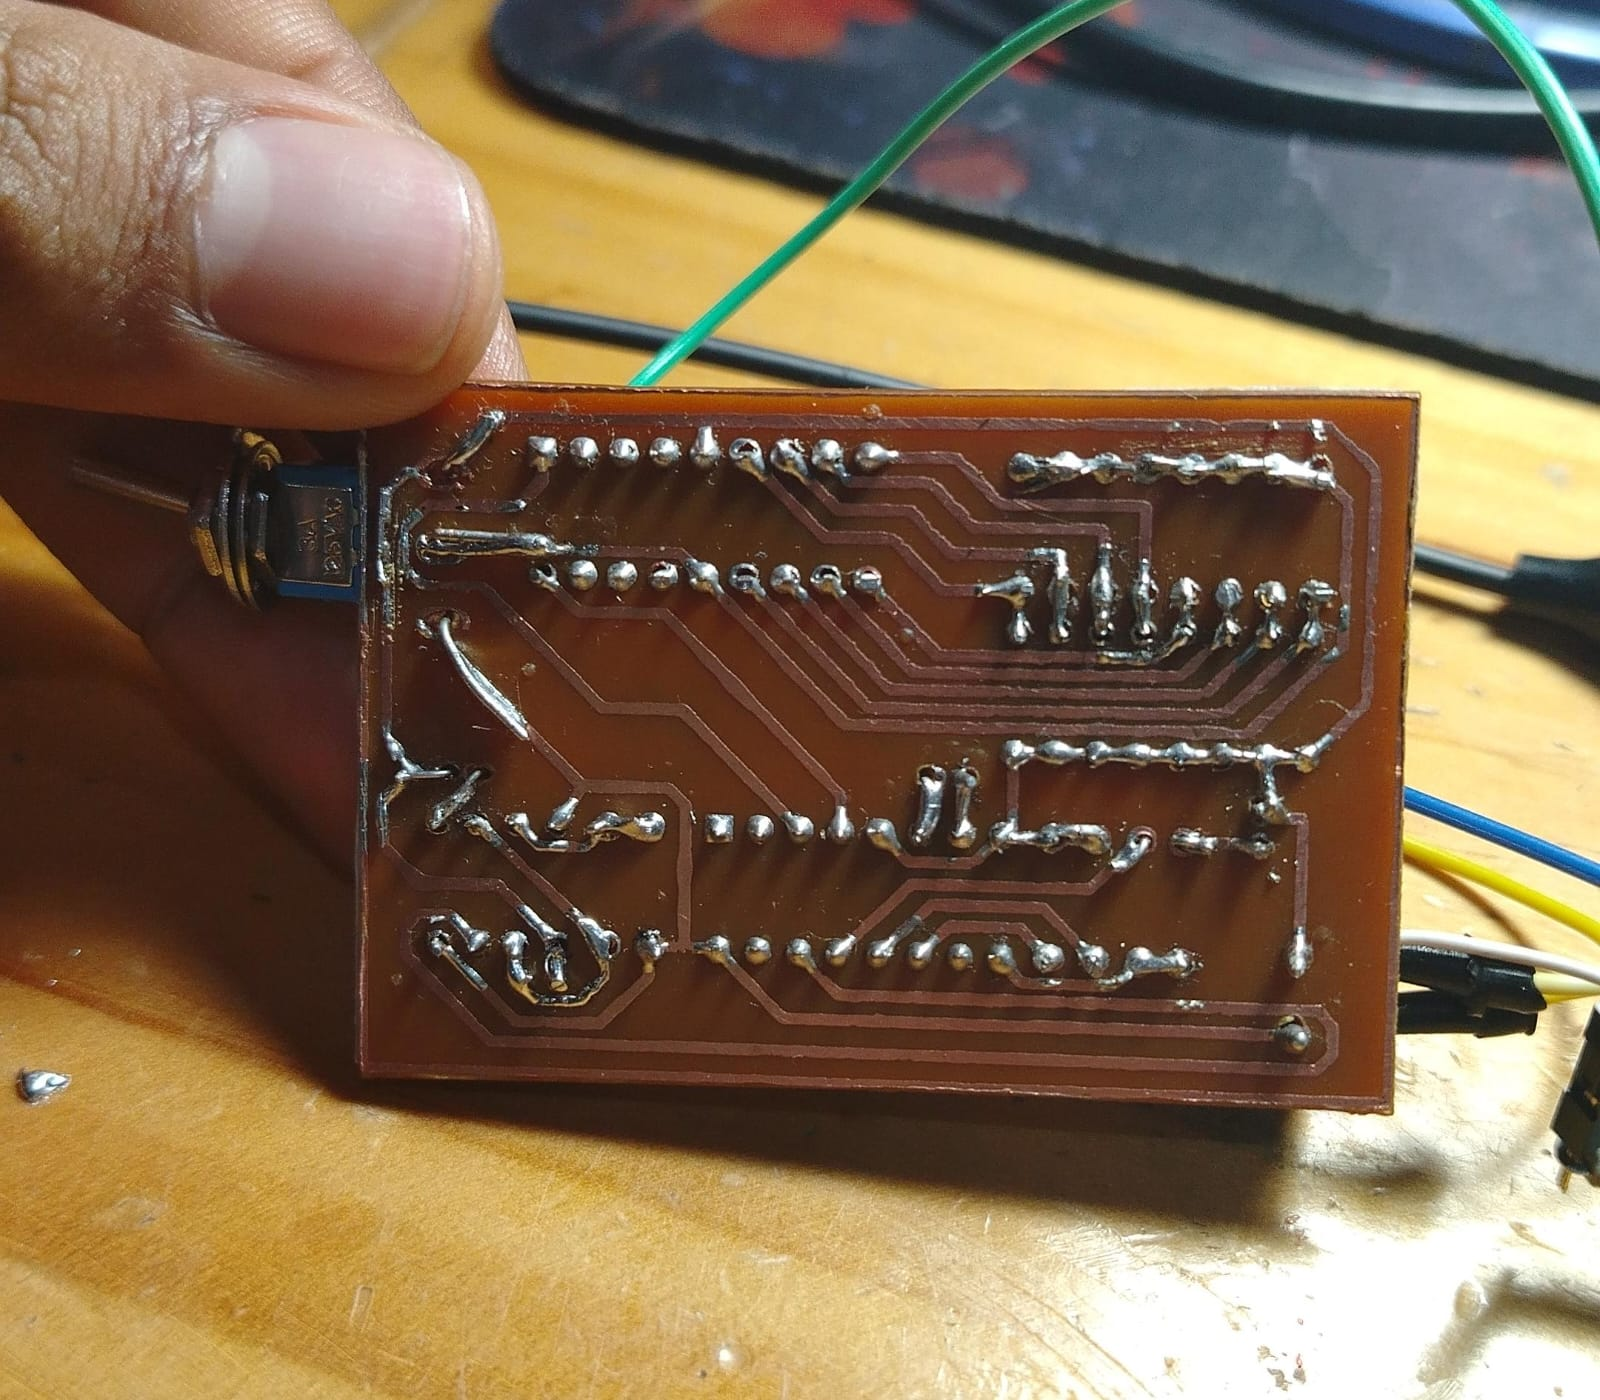
\includegraphics[width=.7\textwidth]{imgs/ANEXO PCB.jpg}
    \caption{PCB IMPRESO}
\end{figure}
\begin{figure}[H]
    \centering
    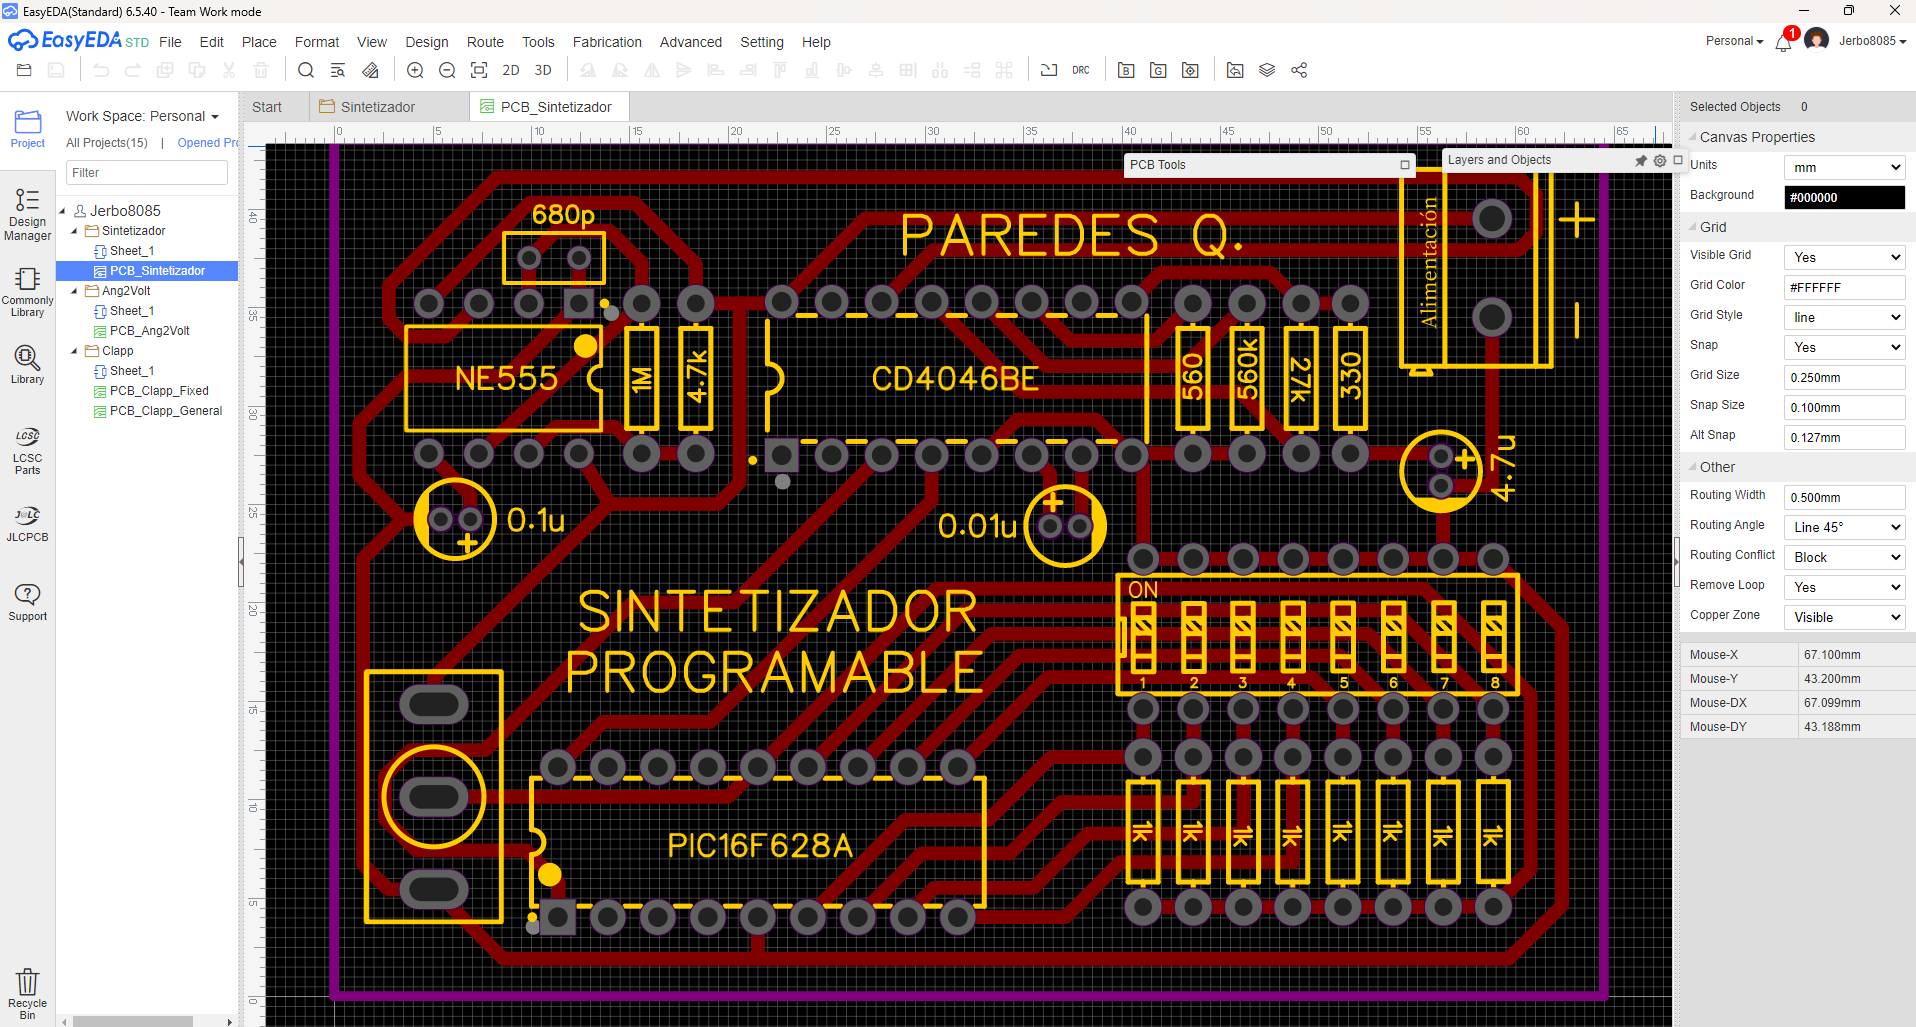
\includegraphics[width=.7\textwidth]{imgs/ANEXO PCB 2.png}
    \caption{PCB DISEÑO}
\end{figure}